\cleardoublepage
\chapter*{Währenddessen im Zoo ~~~ \raisebox{-0.35cm}{
\includegraphics[height=1.0cm]{Bilder/elephant_emoji.png}}}
\addcontentsline{toc}{section}{Währenddessen im Zoo ~~~ \raisebox{-0.25cm}{
\includegraphics[height=0.8cm]{Bilder/elephant_emoji.png}}}
\markboth{Währenddessen im Zoo ~ \raisebox{-0.15cm}{
\includegraphics[height=0.6cm]{Bilder/elephant_emoji.png}}}{\raisebox{-0.15cm}{
\includegraphics[height=0.6cm]{Bilder/elephant_emoji2.png}} ~ Währenddessen im Zoo}
\label{sec:Lektion-4-Zoo}

\marginline{~\\~\\Lektion~1, Seite~\pageref*{sec:Lektion-1-Zoo}\\~\\Lektion~2, Seite~\pageref*{sec:Lektion-2-Zoo}}
\sttpUniversalkasten{Was bisher geschah}{Der städtische Zoo ist an das Softwareunternehmen herangetreten, in dem Sie arbeiten, um zu eruieren, an welchen Stellen Zooabläufe mit Software unterstützt werden könnten und wie der öffentliche Zooauftritt insgesamt digitaler werden kann. Auf einem ersten Brainstorming-Workshop zwischen Softwareteam und Zooteam hat man sich auf die Durchführung eines Vorprojekts geeinigt, in dem der inhaltliche Rahmen für die zukünftige Zusammenarbeit fest\-gelegt werden soll. Erste Diskussionsergebnisse des Workshops zur Domäne Zoo, ihren Abläufen und Aufgaben sowie Überlegungen zum weiteren Vorgehen wurden festgehalten.}

\vspace{1em}


\sttpUniversalkasten{}{
\minisec{Was (ohne unsere Anwesenheit) noch passiert ist}
\vspace{1mm}
Mittlerweile wurden zwei Arbeitsgruppen gebildet. Die Arbeitsgruppe „Domänenmodellierung“ leitet Magnus Fryt, Requirement Engineer im Softwareunternehmen. Von Seiten des Softwareteams nimmt außerdem Paul Klipper (Software\-entwickler) teil, von Seiten des Zoos die beiden Tierpfleger:innen Ruth Temper und Adrian Droschke. Die Tierärztin des Zoos, Wiebke Mellier kann bei Bedarf hinzugeholt werden. Die Arbeitsgruppe „Entwicklungsplanung“ setzt sich zusammen aus Inga Schwab (Leiterin Vorprojekt) und Joris Jonson (Softwarearchitekt) sowie Frau Dr. Walther (Zoodirektorin), Lars Qwert (Marketingchef des Zoos) und Helmut Frohn (oberster Tierpfleger im Zoo). In beiden Arbeitsgruppen haben erste Treffen stattgefunden. \newline
In der AG Entwicklungsplanung hat man sich darauf verständigt, sich im aktuellen Vorprojekt nur ausgewählte Vorhaben der Zoowünsche detaillierter anzusehen, aber grundsätzlich an der Vision einer umfassenden Zoo-Ablaufautomatisierung und Zoo-Digitalisierung festzuhalten -- und dement\-sprechend zukünftiges Erweiterungspotenzial nie aus dem Blick zu verlieren.} 

\clearpage

\minisec{Treffen der Arbeitsgruppe Entwicklungsplanung}

Ausgehend von der von Frau Dr. Walther vorgenommenen Priorisierung der Zoo\-wünsche wird über das weitere Vorgehen diskutiert. 

\marginline{~\\~\\~\\Lektion~2, Seite~\pageref*{text:lektion2_whiteboard_s1}}
% Karteikarte Fallbeispiel Zoo

\sttpKarteikarte{12.5cm}{\sttpKarteikarteSkalierungsfaktor}{\sttpKarteikarteRotierungswinkel}{Überlegungen zum Produkt}%
	{Thema:}{Prioritäten}%
	{Details:}{Am wichtigsten: Umfangreiche Informationen auf der Website zu unseren Tieren und eine Softwareunterstützung beim Futterbestellprozess. \newline Zweite Priorität: die Einbindung der Besucher bei der Namensgebung neugeborener Tiere, ein automatisiertes Patenschaftssystem und der Online-Eintrittskartenverkauf. \newline Weitere Wünsche: Terminverwaltung Tierärzte, komfortableres System zur Tier- und Käfigausleihe.}%
	{Fr. Walther (Zoodirektorin)}
	
	
	


\textbf{Frau Walther:} „Recht dringend ist die Verbesserung des Tierfutter\-bestell\-prozesses. Der läuft aktuell komplett ohne spezialisierte Softwareunterstützung und sehr dezentral, das bindet extrem viel Personalressourcen auf allen Ebenen des Zoos und ist darüber hinaus sehr fehleranfällig. Zudem liegt uns sehr viel daran, in der Region sichtbarer zu werden und auch mehr Besucher:innen anzuziehen. Hierfür benötigen wir eine grundlegende Umgestaltung des digitalen Zoo-Auftritts, perspektivisch auch mit interaktiven Inhalten. Ich habe schon verstanden, dass wir unsere Wunschvorstellungen in diesem Bereich für eine erste Umsetzung noch deutlich eingrenzen müssen. Aber besser als jetzt wird es allemal gehen: Aktuell gibt es nur eine sehr basale Website mit Informationen zu Eintrittspreisen und Öffnungszeiten, noch nicht einmal eine Übersicht der Tierarten im Zoo.“ 

\textbf{Auszug aus dem anschließenden Protokoll:}
\begin{itemize}
	\item Im Fokus werden zwei Vorhaben stehen: 1. Der zukünftige digitale Zoo-Auftritt mit integriertem Tier-Informationssystem (Arbeitstitel: Zoo-Auftritt), 2. Die Begutachtung der aktuellen Zooprozesse im Bereich der Futterbestellung mit dem Ziel, Automatisierungspotenzial aufzuzeigen (Arbeitstitel: Futter-
	\linebreak %%% für Druck
	bestellung).
	\item Die gewünschte Einbindung der Zoobesucher bei der Namensgebung der Tiere soll im Rahmen des Tier-Informationssystems realisiert werden.
	\item Für den Online-Kartenverkauf soll ein auf dem Markt verfügbares konfigurierbares Standardsystem zum Einsatz kommen, das mit dem digitalen Zoo-Auftritt verbunden wird. Das Softwareteam wird den Zoo bei der Auswahl beraten.
	\item Ein automatisiertes Patenschaftssystem wird zunächst zurückgestellt, soll sich aber zukünftig an das Tier-Informationssystem anbinden lassen. Informationen zum Patenschaftssystem des Vogelparks Hohenhausen werden durch den Zoo eingeholt.
	\item Die Ablösung der seit vielen Jahren eingesetzten Softwarelösungen für die Käfig- und Tierausleihe sowie für die Terminverwaltung der Tierärzte wird aktuell nicht angegangen. Zwar gibt es Unzufriedenheiten mit den verfüg\-baren Funktionalitäten, doch sind zahlreiche Arbeitsprozesse mittlerweile an die Beschränkungen der Software angepasst worden, so dass kein prioritärer Handlungsbedarf besteht. 
\end{itemize}

\textbf{Frau Schwab:} „Lassen Sie uns für unsere zwei prioritären Vorhaben konkreter werden: Welche Ziele verfolgen wir?, welche Stakeholder müssen eingebunden werden? und so weiter. Beginnen wir heute noch mit dem Vorhaben Futterbestellung, das ist überschaubarer. Im morgigen Treffen reden wir dann über das Vorhaben Zoo-Auftritt. Zur Futterbestellung: Wir hatten uns ja schon darauf verständigt, dass wir von Seiten unseres Softwareunternehmens jetzt zunächst nur die aktuellen Futter\-bestell\-prozesse im Zoo analysieren, im Anschluss dann einen Vorschlag unterbreiten, an welchen Stellen wir inwiefern Potenzial von Softwareunterstützung sehen und dann nochmal mit der Zooleitung verhandeln, in welchem Umfang wir dieses Projekt in Richtung der Erstellung einer konkreten Anforderungsspezifikation weiterführen. Lassen Sie uns Vision und Ziele aber dennoch schon in Richtung dieser zukünftigen Futterbestellautomatisierung ausrichten und nicht nur auf die aktuell anstehenden Prozess-Begutachtungen.“

\vspace{\baselineskip}

\textbf{Diskussionsergebnisse „Automatisierung Futterbestellung“}

%\vspace{-0.5cm}
{ %% Scope beginnen (damit \renewcommand keine Auswirkung auf andere Karteikarten hat)
	\renewcommand{\sttpKarteikarteSkalierungsfaktor}{0.85}
	
	\begin{addmargin*}[0cm]{-\marginparwidth}
	\begin{addmargin*}[0cm]{-\marginparsep}

	\begin{center}
		\begin{tabular}{ p{8.2cm} p{8.2cm} }
		%\begin{tabular}{ | p{8.2cm} | p{8.2cm} | }
			\vspace{-0.5cm}
			\begin{center}
				\sttpKarteikarte{9.5cm}{\sttpKarteikarteSkalierungsfaktor}{\sttpKarteikarteRotierungswinkel}{Vision}%
{}{Die überwiegend manuell ablaufenden Prozesse der Futterbestellung werden durch eine softwaregestützte Automati\-sierungslösung ersetzt. Die Tierpfleger haben wieder mehr Freiraum für ihre Fachaufgaben in der Versorgung der Tiere. Fehlerhafte Futterbestellungen werden verhindert. Das Futterbestellsystem wird an die Einkaufs- und Abrechnungs\-systeme der Zooverwaltung angebunden.
\begin{flushright}
	 \textnormal{\textsf{\footnotesize{Version 1.0}}}
\end{flushright}
}%
{}{}% Text zum 2. Teil bleibt leer -> keine Anzeige
{}% Ersteller bleibt leer -> keine Anzeige
			\end{center}
	
			\vspace{-0.5cm}
			\begin{center}
				\sttpKarteikarte{9.5cm}{\sttpKarteikarteSkalierungsfaktor}{\sttpKarteikarteRotierungswinkel}{Stakeholder}%
{}{Tierpfleger, Lagerverwalter, Rechnungsabteilung der Zooverwaltung, IT-Abteilung des Zoos, ggf. weitere Abteilungen der Zooverwaltung, ggf. Futterlieferanten}%
{Anmerkungen:}{Sollten sich die Bestellprozesse für verschiedene Tierarten sehr unterscheiden, müssen unbedingt Tierpfleger aus verschiedenen Gebieten einbezogen werden.
\begin{flushright}
	\textnormal{\textsf{\footnotesize{Version 1.0}}}
\end{flushright}
}
{}% Ersteller bleibt leer -> keine Anzeige
			\end{center}
			&
			\vspace{-0.5cm}
			\begin{center}
				\sttpKarteikarte{9.5cm}{\sttpKarteikarteSkalierungsfaktor}{\sttpKarteikarteRotierungswinkel}{Ziele}%
{}{Die Tierpfleger von verwaltungstechnischen Aufgaben befreien \newline 
	Den Futterbestellprozess beschleunigen \newline 
	Den Futterbestellprozess zentralisieren \newline 
	Überblick über den Futterlagerbestand besitzen \newline 
	Minimierung der Futterentsorgung aufgrund über\-schrittener Haltbarkeiten
\begin{flushright}
	\textnormal{\textsf{\footnotesize{Version 1.0}}}
\end{flushright}
}%
{}{}% Text zum 2. Teil bleibt leer -> keine Anzeige
{}% Ersteller bleibt leer -> keine Anzeige



			\end{center}
			\\
		\end{tabular}
	\end{center}

	\end{addmargin*}
	\end{addmargin*}
} %% Scope beenden (um \renewcommand lokal zu halten)

\clearpage

\minisec{Am nächsten Tag}

Auf der Agenda für heute steht das Vorhaben zum digitalen Zoo-Auftritt. Auch hier wird über Vision, Ziele, Stakeholder diskutiert. Die Marketingabteilung des Zoos hat im Vorfeld der Besprechung bei den Kolleg:innen schon Ideen gesammelt (s.~Abb.~\ref{fig:sprechblasen_ideen}), das Softwareteam sich anhand der bisherigen Diskussionen schon mal Gedanken zum Produktumfang und zu Schnittstellen des Systemkontexts gemacht. Man diskutiert und systematisiert.

\begin{figure}[h!]
	\centering
	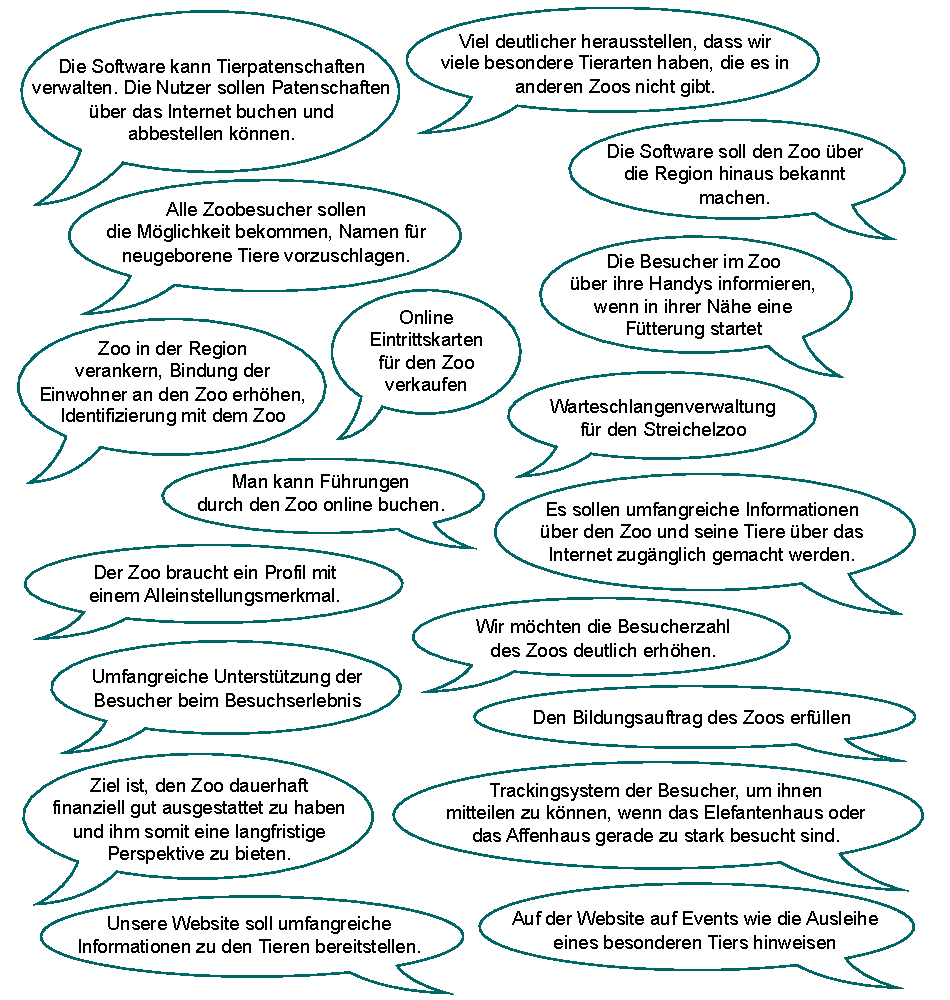
\includegraphics[width=\textwidth]{Bilder/Kapitel-6/sprechblasen_ideen.pdf}
	\caption[Zoo-Ideen zu Motivation, Zielen, Anforderungen etc.]{Unsystematische Mischung von Ideen zu Motivation, Zielen, Anforderungen, \ldots}
	\label{fig:sprechblasen_ideen}
\end{figure}

\clearpage

\minisec{Diskussionsergebnisse „digitaler Zooauftritt“}

{ %% Scope beginnen (damit \renewcommand keine Auswirkung auf andere Karteikarten hat)
	\renewcommand{\sttpKarteikarteSkalierungsfaktor}{0.85}

	\begin{addmargin*}[0cm]{-\marginparwidth}
	\begin{addmargin*}[0cm]{-\marginparsep}
	
	\begin{center}
		\begin{tabular}{ p{8.2cm} p{8.2cm} }
		%\begin{tabular}{ | p{8.2cm} | p{8.2cm} | }
			\vspace{-0.5cm}
			\begin{center}
				\sttpKarteikarte{9.5cm}{\sttpKarteikarteSkalierungsfaktor}{\sttpKarteikarteRotierungswinkel}{Motivation}%
{}{Zoobesuchern ein umfassendes Besuchserlebnis bieten \newline Zoo in der Region verankern und über die Region hinaus bekannt machen \newline Starke Identifikation der Einwohner mit dem Zoo schaffen \newline Den Bildungsauftrag des Zoos erfüllen.}%
{}{}% Text zum 2. Teil bleibt leer -> keine Anzeige
{}% Ersteller bleibt leer -> keine Anzeige
			\end{center}
			&
			\vspace{-0.7cm}
			\begin{center}
				\sttpKarteikarte{9.5cm}{\sttpKarteikarteSkalierungsfaktor}{\sttpKarteikarteRotierungswinkel}{Ziele}%
{}{Alleinstellungsmerkmale des Zoos bekannt machen \newline Steigende Besucherzahlen \newline Zusätzliche Kooperationspartner gewinnen (Studien\-gänge, Schulen, Kindergärten, Bildungsprojekte) und Koopera\-tions\-projekte akquirieren
\begin{flushright}
	\textnormal{\textsf{\footnotesize{Version 1.0}}}
\end{flushright}
}%
{}{}% Text zum 2. Teil bleibt leer -> keine Anzeige
{}% Ersteller bleibt leer -> keine Anzeige
			\end{center}
			\\
			\vspace{-0.5cm}
			\begin{center}
				\sttpKarteikarte{9.5cm}{\sttpKarteikarteSkalierungsfaktor}{\sttpKarteikarteRotierungswinkel}{Produktumfang und Schnittstellen}%
{Produktumfang}{klassische Website-Informationen (Öffnungszeiten, Preise etc.) \newline 
	basales Tier-Informationssystem \newline 
	Komponente zum Tiernamen-Voting \newline 
	spätere Erweiterungen: Auslastungsanzeigen der Zoo\-bereiche (Affenhaus etc.), Event-Benachrichtigungen für Zoo\-besucher
}%
{Schnittstellen}{Anbindung zum detaillierten Tier-Informationssystem der Universität \newline 
	Anbindung an Online-Kartenverkauf \newline 
	zukünftig: Anbindung an Patenschaftssystem, Anbindung an Buchungssystem für Zooführungen
\begin{flushright}
	\textnormal{\textsf{\footnotesize{Version 1.0}}}
\end{flushright}
}
{}{}% Text zum 2. Teil bleibt leer -> keine Anzeige
{}% Ersteller bleibt leer -> keine Anzeige
			\end{center}
			&
			\vspace{-0.5cm}
			\begin{center}
				\sttpKarteikarte{9.5cm}{\sttpKarteikarteSkalierungsfaktor}{\sttpKarteikarteRotierungswinkel}{Stakeholder}%
{}{Marketing-Abteilung, IT-Abteilung, Tierpfleger, Zoo\-besucher, verschiedene Abteilungen der Zooverwaltung, ggf. Zoologie-Studiengang der Universität
\begin{flushright}
	\textnormal{\textsf{\footnotesize{Version 1.0}}}
\end{flushright}
}%
{}{}% Text zum 2. Teil bleibt leer -> keine Anzeige
{}% Ersteller bleibt leer -> keine Anzeige
			\end{center}
			\\
		\end{tabular}
	\end{center}

	\end{addmargin*}
	\end{addmargin*}
} %% Scope beenden (um \renewcommand lokal zu halten)

\textbf{Frau Schwab:} „Der nächste Schritt in beiden Vorhaben ist jetzt die jeweils vorgesehenen Stakeholder zu kontaktieren und mit ihnen weiter an Visionen, Zielen, Produkt\-umfang und so weiter zu arbeiten und dann mit der Anforderungs\-sammlung zu beginnen. Das Vorhaben Futterbestellung geben wir am besten in die Hand der AG Domänenmodellierung, hier müssen ja jetzt hauptsächlich die Prozesse der \mbox{Domäne} diskutiert und dokumentiert werden. Unsere eigene AG Entwicklungs\-planung überführen wir in eine AG Zoo-Auftritt und kümmern uns um dieses Vorhaben.“